\section{Liturgia chrzcielna}

\subsection{Procesja do baptysterium}
\begin{figure}[h]
	\centering
	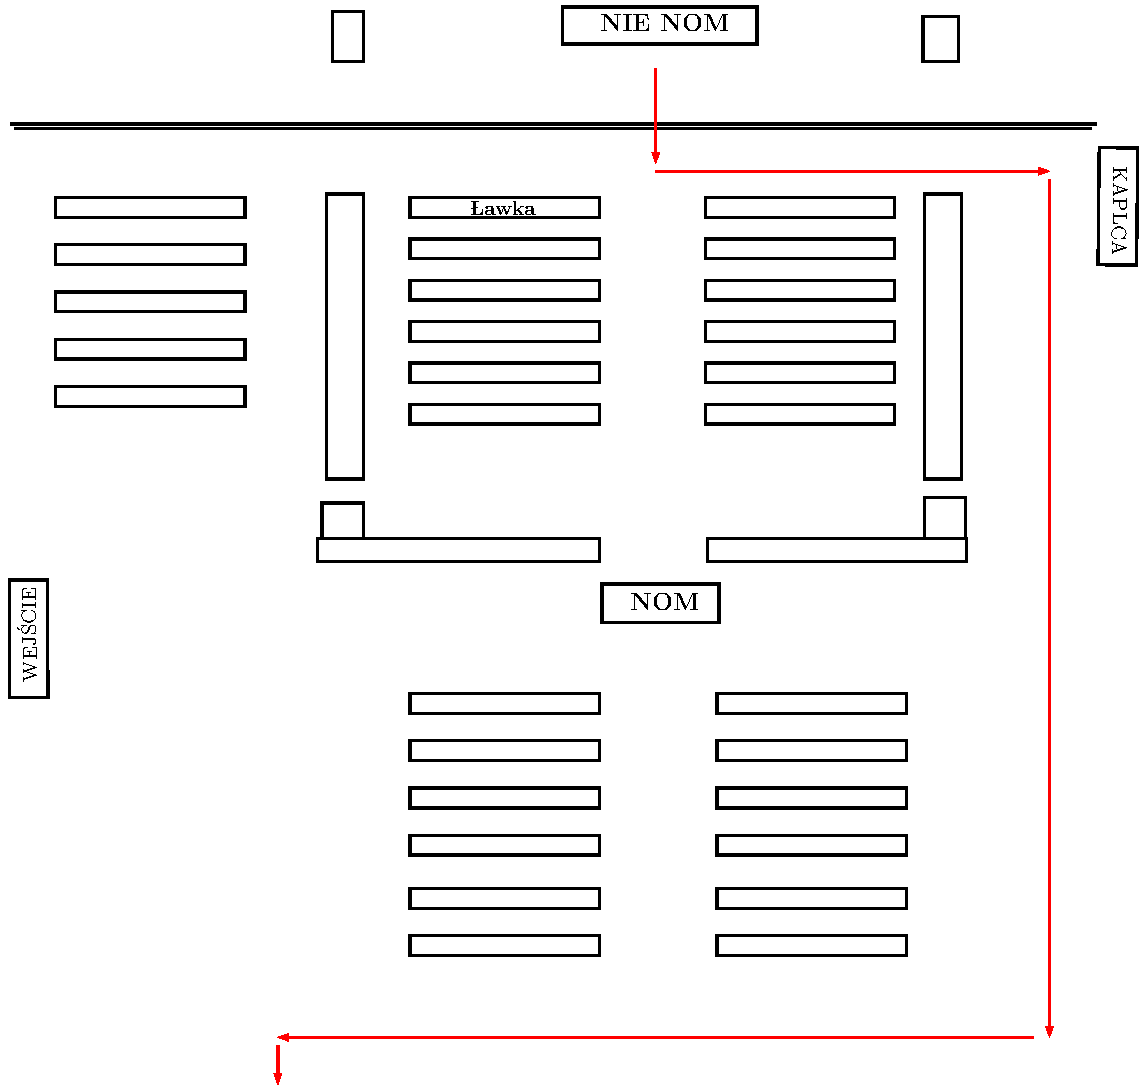
\includegraphics[width=0.6\linewidth]{Figures/Sobota/procesja1.pdf}
	\caption{Droga do chrzcielnicy}
	\label{fig:procesja1}
\end{figure}
\begin{itemize}
	\item po ostatniej oracji \ii~ z \cc1 schodzi krótką drogą na środek ołtarza
	      (po skosie) i ściąga kapę (pomaga \cc2 \footnote{Kapa powinna leżeć w
		      pobliżu, bo zaraz będzie znowu używana})
	\item \ii~ kładzie się krzyżem na poduszkach
	\item gdy to się stanie kantorzy zaczynają śpiew
	      \textit{Litanii do Wszystkich Świętych}
	\item kiedy \ii~ leży krzyżem wszyscy ministranci klęczą
	\item gdy Litania dobiega ku końcowi:
	      \begin{itemize}
		      \item \ii~ wraz z \cc1 wstaje, \cc2 podchodzi z kapą i ubiera \ii
		      \item \aa\aa~ odpalają od świeczki ratunkowej akolitki
		      \item \ding{63} idzie po krzyż procesyjny
		      \item \mm~ idzie po Paschał
	      \end{itemize}
	\item po skończonej Litanii kantorzy podejmują śpiew \textit{Sicut Cervus}
	\item na znak \cc1 formuje się procesja do chrzcielnicy:
	      \begin{center}
		      \cc2~~~\ii~~~\cc1 \smallskip\\
		      ministranci \smallskip\\
		      kantorzy \smallskip\\
		      \aa1~~~\ding{63}~~~\aa2 \smallskip\\
		      \cc3~~~\mm \smallskip\\
		      \downarrow
	      \end{center}
	\item procesja rusza na znak \cc1 (patrz Rys. \ref{fig:procesja1})
\end{itemize}
\subsection{Poświęcenie wody}
\begin{itemize}
	\item po dojściu do kraty:
	      \begin{itemize}
		      \item ministranci funkcyjni wchodzą do baptysterium (patrz Rys.
		            \ref{fig:woda})
		      \item chór też wchodzi do baptysterium, ale głębiej (koło drzwi
		            wejściowych) \footnote{Zostawiając przy tym miejsce dla
			            chóru, który musi stać bliżej chcielnicy} (patrz Rys.
		            \ref{fig:woda})
		      \item \ii, \cc1 i \cc2 stoją przed kratą (jeszcze nie patrz Rys.
		            \ref{fig:woda})
	      \end{itemize}
	\item \ii~ ściąga biret, podaje \cc1, ten odnosi i przynosi księgę z
	      modlitwą. \ii~ czyta kantyk \textit{Sicut Cervus} i czeka, aż chór
	      skończy jego śpiewanie. Następnie odczytuje oracje i po jej skończeniu
	      wchodzi do baptysterium (teraz patrz Rys. \ref{fig:woda})
	      \begin{figure}[h!]
		      \centering
		      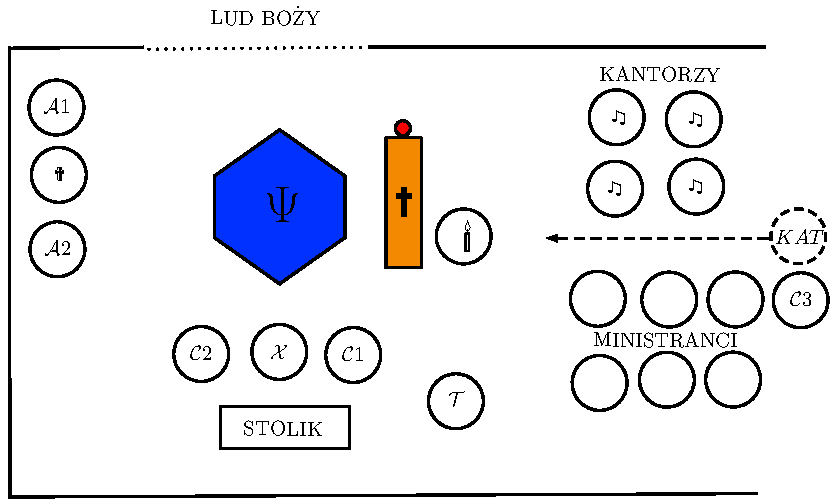
\includegraphics[width=0.7\linewidth]{Figures/Sobota/woda.pdf}
		      \caption{Ustawienie przy chrzcielnicy, $K$ oznacza kantorów, $KAT$
			      oznacza katechumena}
		      \label{fig:woda}
	      \end{figure}
	\item następuje poświęcenie wody chrzcielnej, \cc1 i \cc2 podtrzymują brzegi
	      kapy i pomagają \ii~ podając odpowiednie rzeczy (oleje, ręcznik \dots)
	\item po wszystkich modlitwach (patrz \textit{\nameref{sec:woda}}) następuje
	      zasypanie i okadzenie wody
	\item po okadzeniu wody chrzcielnej \tt~ od razu ucieka bokiem i idzie
	      pomagać \cc3
\end{itemize}
\subsection{Chrzest}
\begin{itemize}
	\item \ii~ zmienia fioletową kapę i stułę na białą
	\item do baptysterium wprowadza się katechumenów z chrzestnymi (stoją oni za
	      ministrantami i kantorami)
	\item \ii~ rozpoczyna dialog z katechumenami
	\item po odpowiedziach na wszystkie pytania, \ii~ nad chrzcielnicą
	      trzykrotnie polewa głowę dziecka lub dorosłego, wypowiadając formułę
	      chrzcielną
	\item \cc1 podaje \ii~ naczynie z Krzyżmem. \ii~ namaszcza ochrzczonych
	      wypowiadając formułę i wyciera kciuk w watę
	\item następnie wręcza się białą szatę oraz płonącą świecę, wypowiadając
	      przepisane formuły
	\item następnie \ii~ wypowiada formułę: \textit{N., vade in pace...}
\end{itemize}
\subsection{Bierzmowanie}
\begin{itemize}
	\item kantorzy podejmują śpiew \textit{O stworzycielu Duchu Przyjdź}
	\item wszyscy oprócz \ii, \cc1 i \cc2 zostają na swoich miejscach, razem z
	      Paschałem
	\item \ii~ w białej kapie z \cc1 i \cc2 oraz katechumenem udają się do
	      kaplicy św. Iwa, oddają rewerencje ołtarzowi i zajmują swoje miejsca:
	      \ii~ siada na faldistorium, \cc\cc~ stoją po bokach a katechumen staje
	      przed stopniami ołtarza po stronie epistoły
	\item przyprowadza się kandydata do ołtarza (razem ze świadkiem), którzy
	      klękają przed stopniem ołtarza
	\item po zakończeniu śpiewu następuje obrzęd bierzmowania (patrz
	      \textit{\nameref{sec:bierz}})
\end{itemize}
\subsection{Odnowienie przyrzeczeń chrzcielnych}
\begin{itemize}
	\item po zakończonym bierzmowaniu kandydat wychodzi z kaplicy
	\item \cc1 podaję \ii~ księgę ze słowami odnowień chrzcielnych (ciągle w
	      kaplicy św. Iwa)
	\item w międzyczasie kiedy \ii~ czyta \cc2 dyskretnie udaje się po
	      kropielnice, ale do kaplicy wchodzi dopiero po kiedy będzie potrzebny
	      (tj. po zakończeniu czytania)
	\item \ii~ razem z \cc1 i \cc2, którzy trzymają kapę, wychodzą z kaplicy do
	      ludzi i następuje pokropienie
	\item w trakcie kropienia śpiewa sie \textit{Com przyrzekł Bogu}
\end{itemize}
\subsection{Procesja do ołtarza głównego} \todo{Trzeba tutaj okadzić Paschał?}
\begin{itemize}
	\item po skończonych obrzędach ustawiamy procesję z powrotem do ołtarza
	      głównego w tym samym porządku co poprzednio (ministranci nie funkcyjni
	      wychodzą zaraz po \aa\aa~ i \ding{63})
	\item kantorzy intonują drugą część \textit{Litanii do Wszystkich Świętych}
	\item po przybyciu do ołtarza \mm~ i \cc3 odstawiają Paschał na swoje
	      miejsce (czyli przy ołtarzu po stornie Ewangelii)
	\item ministranci i \ii~ udają się \underline{bezpośrednio} do kaplicy i się
	      przebierają (\ii~ na biały ornat i stułę, ministranci na koronkowe
	      komże)
\end{itemize}
\subsection{Przygotowanie Mszy}
\begin{itemize}
	\item jak ministranci są jeszcze przy chrzcielnicy
	      \begin{itemize}
		      \item odstawić stojak na paschał na stronę ewangelii
		      \item ustawić kolumnę pod figurę Zmartwychwstałego po stronie
		            epistoły
		      \item odstawić pulpit do kaplicy
		      \item powiesić stułę na krzyż
		      \item ustawić relikwie, kwiaty
		      \item zmienić sedille
		      \item zdjąć {\color{violet} fioletową} zasłonę z antypendium
		      \item na razie \underline{nie} rozkładać obrusów!!!
		            \todo{tak było w instrukcji Marka ;) To można tutaj rozłożyć ten obrus?}
	      \end{itemize}
	\item jak ministranci są już w kaplicy
	      \begin{itemize}
		      \item \textbf{zapalić świece} (to zrobić jako pierwsze bo
		            najdłużej zajmuje)
		      \item rozłożyć obrus
	      \end{itemize}
\end{itemize}

